\documentclass[10pt,twocolumn,letterpaper]{article}

\usepackage{cvpr}
\usepackage{times}
\usepackage{epsfig}
\usepackage{graphicx}
\usepackage{amsmath}
\usepackage{amssymb}

% Include other packages here, before hyperref.

% If you comment hyperref and then uncomment it, you should delete
% egpaper.aux before re-running latex.  (Or just hit 'q' on the first latex
% run, let it finish, and you should be clear).
\usepackage[breaklinks=true,bookmarks=false]{hyperref}

\cvprfinalcopy % *** Uncomment this line for the final submission

\def\cvprPaperID{****} % *** Enter the CVPR Paper ID here
\def\httilde{\mbox{\tt\raisebox{-.5ex}{\symbol{126}}}}

% Pages are numbered in submission mode, and unnumbered in camera-ready
%\ifcvprfinal\pagestyle{empty}\fi
\setcounter{page}{1}
\begin{document}

%%%%%%%%% TITLE
\title{Sketch Recognition Classification}

\author{Wayne Lu\\
Stanford University \\
{\tt\small waynelu@stanford.edu}
% For a paper whose authors are all at the same institution,
% omit the following lines up until the closing ``}''.
% Additional authors and addresses can be added with ``\and'',
% just like the second author.
% To save space, use either the email address or home page, not both
\and
Elizabeth Tran\\
Stanford University\\
{\tt\small eliztran@stanford.edu}
}

\maketitle
%\thispagestyle{empty}

%%%%%%%%% ABSTRACT
\begin{abstract}
 Automatic recognition of sketches differs from other areas of image classification because sketches of the same object can vary based on artistic style and drawing ability. In addition, sketches are less detailed and thus harder to distinguish than photographs. Using a publicly available dataset of 20,000 sketches across 250 classes from Eitz et al. ~\cite{eitz2012hdhso}, we are applying ConvNets in order to improve performance over traditional multi-class support vector classifiers (SVMs) using by experimenting with different architecture methods, such as quadrant pooling and fine tuning, and hyperparameters to asses the overall performance of our proposed model. 
\end{abstract}

%%%%%%%%% BODY TEXT
\section{Introduction}
Sketching is one of the primary methods people use to communicate visual information. Since the era of primitive cave paintings, humans have used simple illustrations to represent real-world objects and concepts. Sketches are often abstract and stylized, varying based on artistic ability and style. In addition, sketches emphasize defining characteristics of real-world objects and ignore features which are either less important or more difficult to draw. For example, texture is almost never rendered unless it is important for recognition, such as the spikes on a hedgehog. In this way, sketches can be interpreted as a distillation of human visual recognition schemas.

The sketch recognition problem differs from traditional photographic image classification. First, sketches are less visually complex than photographs. Whereas color photographs have three color channels per pixel, sketches are encoded as either black-and-white or grayscale. Photographs contain visual information throughout the image whereas sketches consist primarily of blank space. Second, sketches and photographs have different sources of intraclass variation. Whereas photographic image classification faces obstacles such as camera angle, occlusion, and illumination, photographs are still grounded in reality. On the other hand, sketches differ based on artistic style, which is unique to every artist. While people can agree on what an object looks like, how they ultimately render the object can vary significantly.

In this paper, we explore the use of deep convolutional neural network architectures for sketch recognition.

\section{Related Work}
Since SketchPad ~\cite{sutherland1964sketchpad}, sketch recognition has introduced sketching as a means of human computer interaction. Computer vision has since tried different approaches to achieve better results in multiple application areas. Eitz et al. ~\cite{eitz2012hdhso} were able to demonstrate classification rates can be achieved for computational sketch recognition by using local feature vectors, bag of features sketch representation and SVMs to classify sketches. Schneider et al. ~\cite{schneider2014sketch} then modified the benchmark proposed by Eitz et al ~\cite{eitz2012hdhso} by making it more focused on how the image should like, rather than the original drawing intention, and they also used SIFT, GMM based on Fisher vector encoding, and SVMs to achieve sketch recognition. 




%-------------------------------------------------------------------------
\section{Dataset}
Eitz et al. ~\cite{eitz2012hdhso} defined a taxonomy of 250 object categories gathered from 20,000 human sketches (TU-Berlin sketch benchmark). The dataset has a total of 250 classes, and it is split into three categories: exhaustive, recognizable, and specific. Images are available as 1111x1111 px PNG files, which we have resized to 128x128 px grayscale images.

\begin{figure}[h]
	\begin{center}
	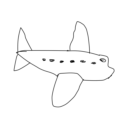
\includegraphics[width=0.5\linewidth]{airplane}
	\caption{Example sketch from TU Berlin dataset.}
	\end{center}
\end{figure}


%-------------------------------------------------------------------------
\section{Approach}
We first preprocess the dataset to produce 128x128 px images. The original images are rescaled from 1111x1111px to 128x128px via bilinear interpolation. The resized images are then read into memory as grayscale 128x128 arrays.

Our approach follows a fairly standard image classification pipeline. Image arrays are fed into a convolution neural network with the final output being fed to a 250-unit fully connected layer to generate logits for each class. We then apply a softmax loss function to the logits and optimize the loss using the Adam algorithm.

At the moment, we are still experimenting with ConvNet architectures. We have been exploring novel architectures from scratch using convolutional, batch normalization, and pooling layers, but as of this writing, nothing has been very successful. Due to time constraints, we will change our approach after this milestone to using existing architectures such as AlexNet or ResNet as starting points to explore from. We will likely also employ the method of image distortion used by Seddati et al. ~\cite{seddati2015deepsketch} to improve generalization.

\begin{table}[h]
\begin{center}
\begin{tabular}{|l|c|}
\hline
Method & mAP \\
\hline\hline
SIFT-varient + BoF + SVM  ~\cite{eitz2012hdhso}  &  56 \\
IDM + SVM ~\cite{yesilbek2015svm} & 71.30 \\
ConvoNet ~\cite{seddati2015deepsketch}  & 75.42\\
ConvoNet ~\cite{seddati2016deepsketch} & 77.69\\
\hline
\end{tabular}
\end{center}
\caption{Performance comparison of our models versus other methods.}
\end{table}


%-------------------------------------------------------------------------
\section{Experiments}
The first model that we train is a single sketch CNN. We would pass an individual sketch through the CNN. The CNN has 3 convolutional layers consisting of 128 x 128, 64 x 64, and 32 x 32 filters respectively. Each convolutional layer is followed by a batch normalization, ReLU (Rectified Linear Unit) activation function, and a 2 x 2 max pooling. After the convolutional layer is a fully-connected layer, we use cross  entropy as a cost function. With this model, we were able to achieve a test accuracy of 0.004. 

In order to improve our network, we are going to try different parameters such as CNN with different levels of regularization, CNN with dropout, CNN with data augmentation, and CNN with dropout and data augmentation. 

%-------------------------------------------------------------------------
{\small
\bibliographystyle{ieee}
\bibliography{milestone}
}

\end{document}
